%%%%%%%%%%%%%%%%%%%%%%%%%%%%%%%%%%%%%%%%%%%%%%%%%%%%%%%%%%%%%%%%%%
%%%%%%%%%%%%%%%%%%%%%%%%%%%%%%%%%%%%%%%%%%%%%%%%%%%%%%%%%%%%%%%%%%
\chapter{Numerische Methoden}
\label{sec:numerical}
%%%%%%%%%%%%%%%%%%%%%%%%%%%%%%%%%%%%%%%%%%%%%%%%%%%%%%%%%%%%%%%%%%
%%%%%%%%%%%%%%%%%%%%%%%%%%%%%%%%%%%%%%%%%%%%%%%%%%%%%%%%%%%%%%%%%%

Numerische Methoden spielen in der Datenanalyse u.\,a.\ deswegen eine wichtige Rolle, weil nur in Spezialfällen geschlossene Formeln für die Parameterschätzung existieren, die zu einer bestmöglichen Passung eines statistischen Modells für beobachtete Daten führt. Der Einsatz numerischer Methoden bleibt dem Anwender aber verborgen, weil die typischerweise eingesetzten Funktionen zur Modellanpassung zwar intern auf solchen Methoden beruhen, sie die gewählten Algorithmen dem Anwender aber nicht unmittelbar offen legen.

Gemein ist allen numerischen Methoden, dass die von ihnen bestimmten Ergebnisse anders als analytische Lösungen von begrenzter numerischer Genauigkeit und auch nicht immer optimal sind. Auch ist es möglich, dass gar keine Lösungen gefunden werden, obwohl sie eigentlich existieren. Um numerische Methoden in eigenen maßgeschneiderten Auswertungen einsetzen zu können, sollte man sich daher auch mit den technischen Hintergründen vertraut machen. Details beschreiben \citeA{Bloomfield2014} und \citeA{Nash2014a}, Hinweise auf relevante Zusatzpakete liefert der Abschnitt \emph{Numerical Mathematics} der CRAN Task Views \cite{CRANtvNumerical}.\footnote{Wichtige numerische Methoden für die lineare Algebra erläutern Abschn.\ \ref{sec:matSolve} und \ref{sec:matDecomp}. Für Pakete zur Bearbeitung der hier nicht besprochenen gewöhnlichen oder partiellen Differentialgleichungen vgl.\ den entsprechenden Abschnitt \emph{Differential Equations} \cite{CRANtvDiffEq} der CRAN Task Views.}

In den folgenden Abschnitten müssen an vielen Stellen selbst Funktionen definiert werden. Die dafür notwendigen Grundlagen vermittelt Abschn.\ \ref{sec:function}.

%%%%%%%%%%%%%%%%%%%%%%%%%%%%%%%%%%%%%%%%%%%%%%%%%%%%%%%%%%%%%%%%%%
%%%%%%%%%%%%%%%%%%%%%%%%%%%%%%%%%%%%%%%%%%%%%%%%%%%%%%%%%%%%%%%%%%
\section{Daten interpolieren und glätten}
\label{sec:interpolate}
%%%%%%%%%%%%%%%%%%%%%%%%%%%%%%%%%%%%%%%%%%%%%%%%%%%%%%%%%%%%%%%%%%
%%%%%%%%%%%%%%%%%%%%%%%%%%%%%%%%%%%%%%%%%%%%%%%%%%%%%%%%%%%%%%%%%%

\index{Daten!interpolieren}
R verfügt über verschiedene vorbereitete Möglichkeiten, zwischen gegebenen Datenpunkten im zweidimensionalen Raum zu interpolieren und Daten zu fitten. Hierbei werden Datenpunkte generiert, die horizontal und vertikal zwischen den bestehenden plaziert sind und diese i.\,S.\ einer zugrundeliegenden Funktion ergänzen. Für Möglichkeiten zum Anpassen verschiedener Funktionsfamilien s.\ Abschn.\ \ref{sec:fitDistr}.

%%%%%%%%%%%%%%%%%%%%%%%%%%%%%%%%%%%%%%%%%%%%%%%%%%%%%%%%%%%%%%%%%%
%%%%%%%%%%%%%%%%%%%%%%%%%%%%%%%%%%%%%%%%%%%%%%%%%%%%%%%%%%%%%%%%%%
\subsection{Lineare Interpolation}
\label{sec:linearInter}
%%%%%%%%%%%%%%%%%%%%%%%%%%%%%%%%%%%%%%%%%%%%%%%%%%%%%%%%%%%%%%%%%%
%%%%%%%%%%%%%%%%%%%%%%%%%%%%%%%%%%%%%%%%%%%%%%%%%%%%%%%%%%%%%%%%%%

\lstinline!approx()!\index[func]{approx()@\lstinline{approx()}} interpoliert linear zwischen Datenpunkten (Abb.\ \ref{fig:interpol}).
\begin{lstlisting}
approx(x=<<x-Koordinaten>>, y=<<y-Koordinaten>>,
       method="<<Interpolationsmethode>>", n=<<Anzahl>>)
\end{lstlisting}

Die $(x, y)$-Koordinaten der Datenpunkte sind für \lstinline!x! und \lstinline!y! in Form von Vektoren derselben Länge zu übergeben. Mit dem Argument \lstinline!method! wird kontrolliert, wie die Interpolation erfolgt -- \lstinline!"linear"! bewirkt eine lineare Interpolation. Mit \lstinline!"constant"! erhalten alle interpolierten Punkte die $y$-Koordinate des in horizontaler Richtung vorangehenden Datenpunkts. Wie viele Punkte der interpolierten Funktion erzeugt werden sollen, bestimmt das Argument \lstinline!n!. Die Ausgabe von \lstinline!approx()! besteht aus einer Liste mit den Komponenten \lstinline!x! und \lstinline!y!, den Vektoren der $(x, y)$-Koordinaten der interpolierten Punkte.\footnote{\lstinline!approxfun()!\index[func]{approxfun()@\lstinline{approxfun()}} gibt stattdessen eine Funktion zurück, die $x$-Koordinaten akzeptiert und $y$-Koordinaten ausgibt, so dass die ursprünglichen Daten interpoliert werden. \lstinline!approxfun()! besitzt dieselben Argumente wie \lstinline!approx()! bis auf die nicht benötigte Angabe \lstinline!n!.}
\begin{lstlisting}
> xOne     <- 1:9                                       # x-Koordinaten
> yOne     <- rnorm(9)                                  # y-Koordinaten
> ptsLin   <- approx(xOne, yOne, method="linear")       # linear
> ptsConst <- approx(xOne, yOne, method="constant")     # konstant

# linkes Diagramm
> plot(xOne, yOne, pch=19, cex=2, main="Datenpunkte interpolieren")
> points(ptsLin,   pch=16, col="red",  lwd=1.5)
> points(ptsConst, pch=22, col="blue", lwd=1.5)
> legend(x="topright", c("Daten", "linear", "konstant"),
+         pch=c(19, 16, 22), col=c("black", "red", "blue"))
\end{lstlisting}

\begin{figure}[ht]
\centering
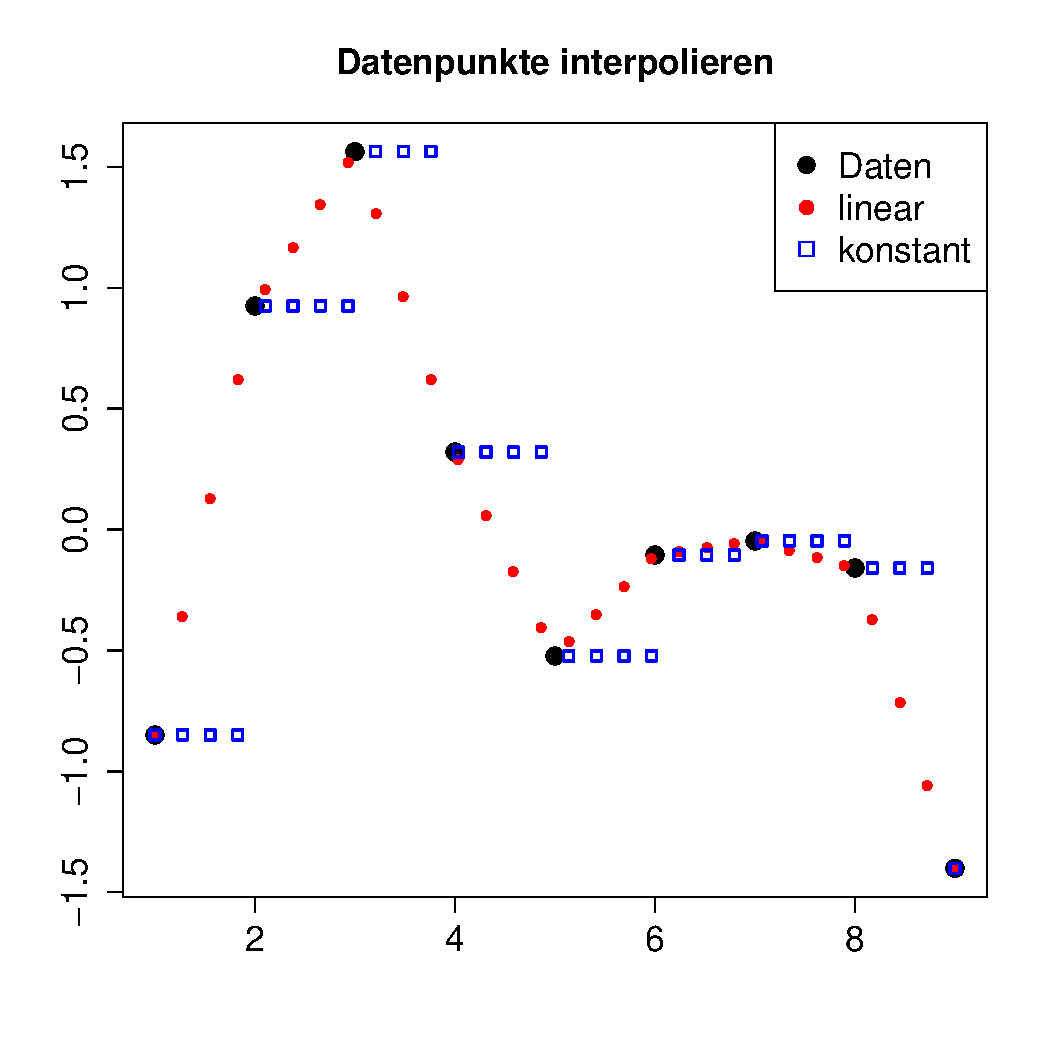
\includegraphics[width=8cm]{interpol}
\vspace*{-1.5em}
\caption{Lineare und konstante Interpolation von Daten}
\label{fig:interpol}
\end{figure}

%%%%%%%%%%%%%%%%%%%%%%%%%%%%%%%%%%%%%%%%%%%%%%%%%%%%%%%%%%%%%%%%%%
%%%%%%%%%%%%%%%%%%%%%%%%%%%%%%%%%%%%%%%%%%%%%%%%%%%%%%%%%%%%%%%%%%
\subsection{Splines}
\label{sec:splines}
%%%%%%%%%%%%%%%%%%%%%%%%%%%%%%%%%%%%%%%%%%%%%%%%%%%%%%%%%%%%%%%%%%
%%%%%%%%%%%%%%%%%%%%%%%%%%%%%%%%%%%%%%%%%%%%%%%%%%%%%%%%%%%%%%%%%%

\index{Grafik!interpolieren}
\index{splines}
Splines sind parametrisierte Kurven, die sich dafür eignen, zwischen Werten glatt zu interpolieren bzw.\ Daten durch glatte Kurven zu approximieren, wenn keine theoretisch motivierte Funktion bekannt ist. Kubische splines können mit\index[func]{spline()@\lstinline{spline()}} \lstinline!spline()! und\index[func]{smooth.spline()@\lstinline{smooth.spline()}} \lstinline!smooth.spline()! erzeugt werden: Während die von \lstinline!spline()! ermittelten Punkte dabei auf einer Kurve durch alle vorhandenen Datenpunkte liegen, ist dies für die von \lstinline!smooth.spline()! berechnete Kurve nicht der Fall. Hier lässt sich die Kurve über das Argument \lstinline!spar! (\emph{smoothing parameter}) in ihrer Glattheit, d.\,h.\ in dem Ausmaß ihrer Variation kontrollieren. Dadurch wird auch bestimmt, wie nah sie an den Datenpunkten liegt.

\lstinline!spline()! gibt eine Liste mit den $(x, y)$-Koordinaten in den Komponenten \lstinline!x! und \lstinline!y! aus.\footnote{\lstinline!splinefun()!\index[func]{splinefun()@\lstinline{splinefun()}} gibt stattdessen eine Funktion zurück, die $x$-Koordinaten akzeptiert und $y$-Koordinaten ausgibt, so dass die ursprünglichen Daten interpoliert werden. \lstinline!splinefun()! besitzt dieselben Argumente wie \lstinline!spline()! bis auf die nicht benötigte Angabe \lstinline!n!.} Das Ergebnis von \lstinline!smooth.spline()! ist ein Objekt, mit dem über \lstinline!predict()! die interpolierten $y$-Koordinaten für neue $x$-Koordinaten erzeugt werden können.

\lstinline!xspline()!\index[func]{xspline()@\lstinline{xspline()}} stellt weitere splines bereit, mit denen nicht nur Funktionswerte interpoliert, sondern allgemein über \emph{Kontrollpunkte} beliebige, auch geschlossene und sich überschneidende Formen angenähert werden können (Abb.\ \ref{fig:splines}). Sofern gewünscht zeichnet \lstinline!xspline()! das Ergebnis direkt in ein Diagramm ein.\footnote{Für weitere Spline-Typen, etwa monotone splines, vgl.\ \lstinline!help(package="splines")!.}
\begin{lstlisting}
> ord <- order(xTwo)                      # für geordnete x-Koordinaten
> idx <- seq(8, 88, by=20)                # wähle 4 Kontrollpunkte
> xspline(xTwo[ord][idx], yTwo[ord][idx], c(1, -1, -1, 1, 1),
+         border="darkgreen", lwd=2, open=FALSE)

> legend(x="topleft", c("Daten", "Loess span 1/3", "Loess span 2/3",
+        "xspline"), pch=c(19, NA, NA, NA), lty=c(NA, 1, 1, 1),
+        col=c("black", "red", "blue", "darkgreen"))

# rechtes Diagramm
> plot(xOne, yOne, pch=19, cex=1.5, main="Splines")  # Daten
> ptsSpline <- spline(xOne, yOne, n=201)             # kubischer spline

# smoothing splines unterschiedlicher Glattheit
> smSpline1 <- smooth.spline(xOne, yOne, spar=0.25)  # recht variabel
> smSpline2 <- smooth.spline(xOne, yOne, spar=0.35)  # mittel variabel
> smSpline3 <- smooth.spline(xOne, yOne, spar=0.45)  # recht glatt

# neue x-Koordinaten, auf die splines angewendet werden
> ptsX      <- seq(1, 9, length.out=201)
> ptsSmSpl1 <- predict(smSpline1, ptsX)
> ptsSmSpl2 <- predict(smSpline2, ptsX)
> ptsSmSpl3 <- predict(smSpline3, ptsX)

# Linien einzeichnen
> lines(ptsSpline, col="darkgray", lwd=2)
> matlines(x=ptsX, y=cbind(ptsSmSpl1$y, ptsSmSpl2$y, ptsSmSpl3$y),
+          col=c("blue", "green", "orange"), lty=1, lwd=2)

> legend(x="topright", c("data", "spline", "spar=0.3", "spar=0.4",
+        "spar=0.5"), pch=c(19, NA, NA, NA, NA), lty=c(NA, 1, 1, 1, 1),
+        col=c("black", "darkgray", "blue", "green", "orange"))
\end{lstlisting}

\begin{figure}[ht]
\centering
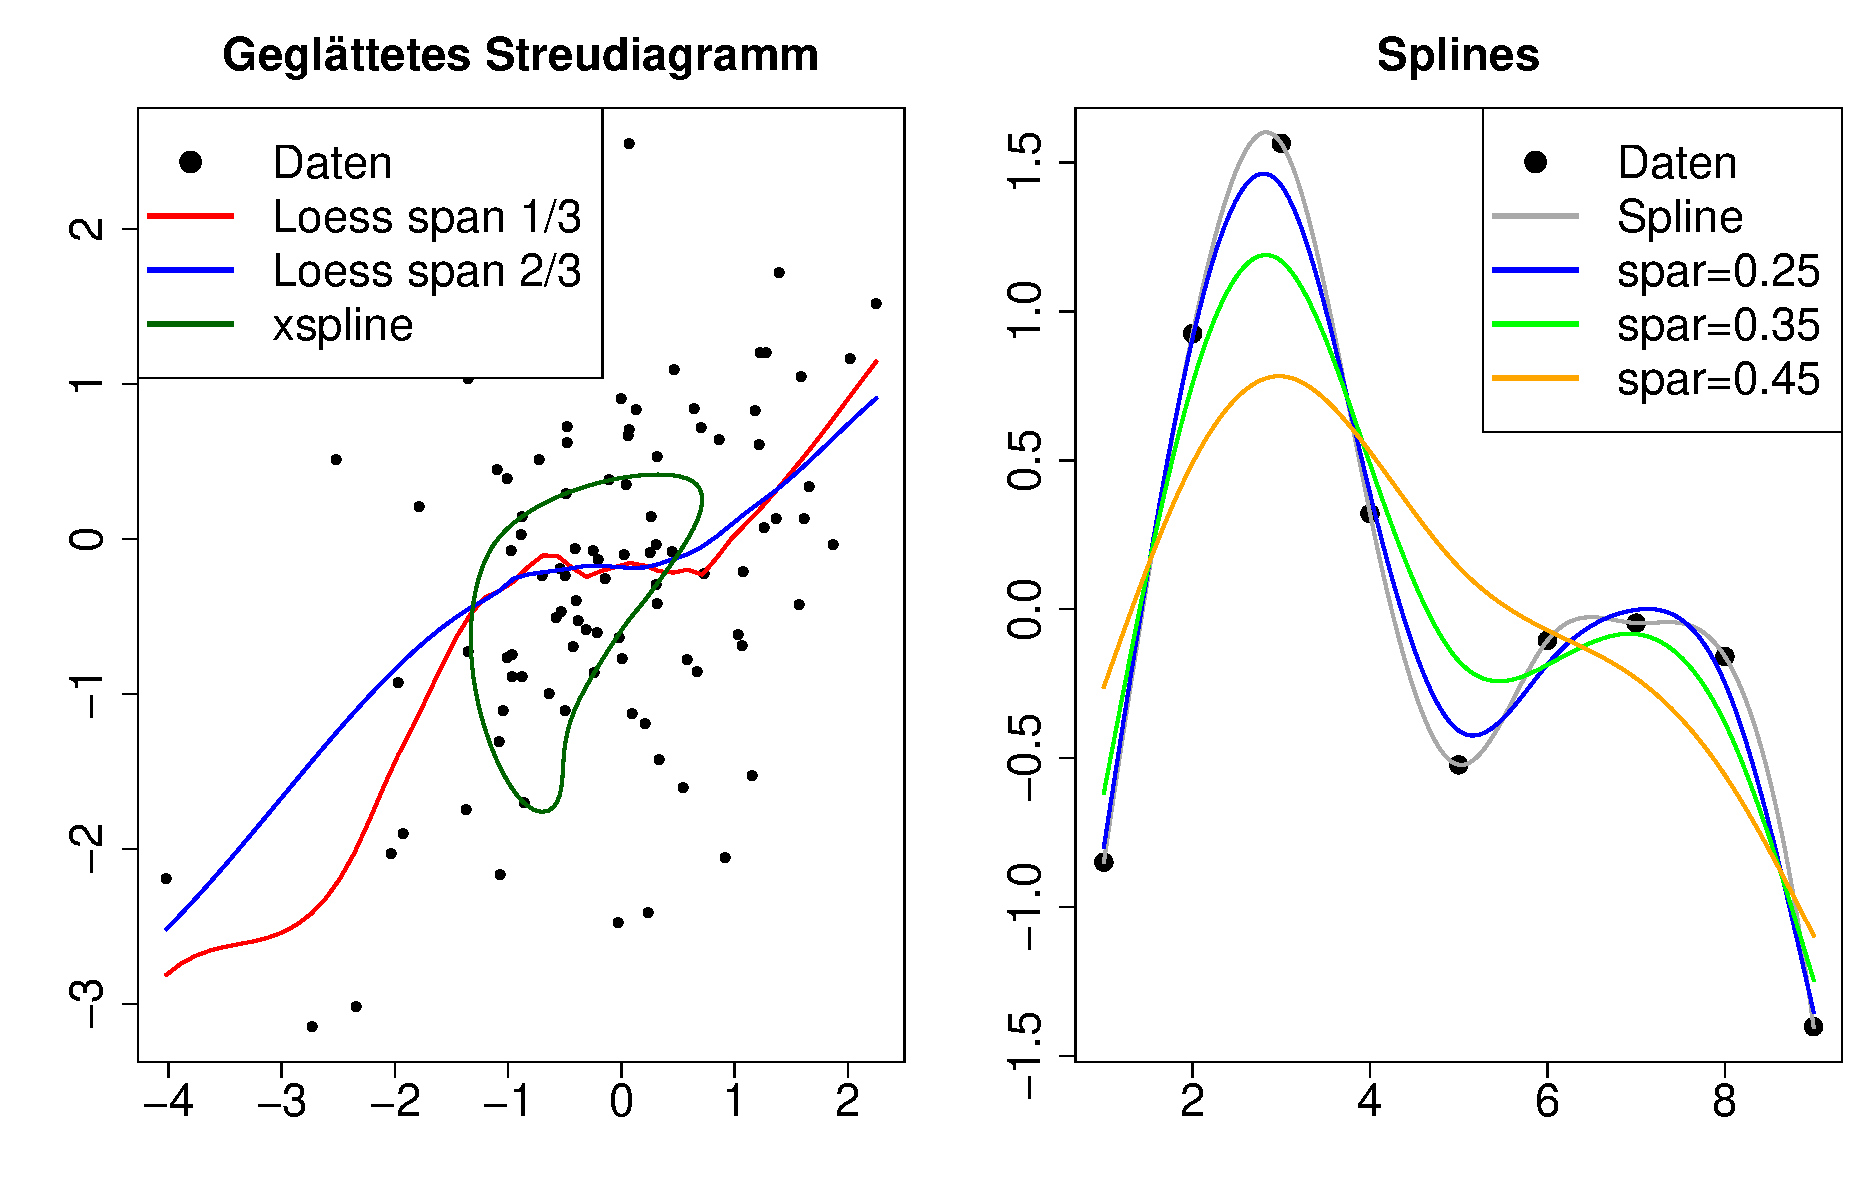
\includegraphics[width=12.5cm]{splines}
\vspace*{-1.5em}
\caption{Polynomiale Glätter sowie unterschiedlich glatte splines}
\label{fig:splines}
\end{figure}

%%%%%%%%%%%%%%%%%%%%%%%%%%%%%%%%%%%%%%%%%%%%%%%%%%%%%%%%%%%%%%%%%%
%%%%%%%%%%%%%%%%%%%%%%%%%%%%%%%%%%%%%%%%%%%%%%%%%%%%%%%%%%%%%%%%%%
\subsection{LOESS-Glätter}
\label{sec:loess}
%%%%%%%%%%%%%%%%%%%%%%%%%%%%%%%%%%%%%%%%%%%%%%%%%%%%%%%%%%%%%%%%%%
%%%%%%%%%%%%%%%%%%%%%%%%%%%%%%%%%%%%%%%%%%%%%%%%%%%%%%%%%%%%%%%%%%

\index{Grafik!Glätter}
Um $(x, y)$-Streudiagramme nonparametrisch durch glatte Kurven zu approximieren, existieren verschiedene Glätter, die auf lokal gewichteten Polynomen basieren -- darunter die in\index[func]{loess()@\lstinline{loess()}} \lstinline!loess()! und\index[func]{loess.smooth()@\lstinline{loess.smooth()}} \lstinline!loess.smooth()! implementierten (Abb.\ \ref{fig:splines}).\footnote{Das im Basisumfang enthaltene Paket \lstinline!KernSmooth!\index[pack]{KernSmooth@\lstinline{KernSmooth}|textbf} \cite{Wand2013} stellt mit \lstinline!locpoly()!\index[func]{locpoly()@\lstinline{locpoly()}} eine weitere Alternative bereit, deren optimale Bandbreite über \lstinline!dpill()!\index[func]{dpill()@\lstinline{dpill()}} aus demselben Paket berechnet werden kann.}
\begin{lstlisting}
loess(<<Modellformel>>, data=<<Datensatz>>, span=<<Bandbreite>>)
loess.smooth(x=<<x-Koordinaten>>, y=<<y-Koordinaten>>, span=<<Bandbreite>>)
\end{lstlisting}

Die $(x, y)$-Koordinaten der Datenpunkte sind in \lstinline!loess()! als Modellformel \lstinline!y ~ x! zu spezifizieren, wobei ggf.\ der die Variablen enthaltende Datensatz für \lstinline!data! genannt werden muss. In \lstinline!loess.smooth()! lassen sich die Koordinaten für \lstinline!x! und \lstinline!y! in Form von Vektoren derselben Länge übergeben. Das Argument \lstinline!span! gibt die Bandbreite des Glätters als Anteil der Punkte an, deren Position in jedem geglätteten Wert berücksichtigt wird. Größere Anteile bewirken dabei glattere Interpolationen (Voreinstellung ist $\frac{2}{3}$).

Das Ergebnis von \lstinline!loess()! ist ein Objekt, mit dem über \lstinline!predict()! die interpolierten $y$-Koordinaten für neue $x$-Koordinaten erzeugt werden können. \lstinline!loess.smooth()! gibt eine Liste mit den Komponenten \lstinline!x! und \lstinline!y! zurück, den Vektoren der $(x, y)$-Koordinaten der interpolierten Punkte.
\begin{lstlisting}
# mittleres Diagramm
> xTwo  <- rnorm(100)                                   # x-Koordinaten
> yTwo  <- 0.4 * xTwo + rnorm(100, 0, 1)                # y-Koordinaten
> ptsL1 <- loess.smooth(xTwo, yTwo, span=1/3)           # weniger glatt
> ptsL2 <- loess.smooth(xTwo, yTwo, span=2/3)           # glatter
> plot(xTwo, yTwo, xlab=NA, ylab=NA, pch=16,
+      main="Geglättetes Streudiagramm")

> lines(ptsL1, lwd=2, col="red")            # LOESS-Glätter einzeichnen
> lines(ptsL2, lwd=2, col="blue")
\end{lstlisting}

%%%%%%%%%%%%%%%%%%%%%%%%%%%%%%%%%%%%%%%%%%%%%%%%%%%%%%%%%%%%%%%%%%
%%%%%%%%%%%%%%%%%%%%%%%%%%%%%%%%%%%%%%%%%%%%%%%%%%%%%%%%%%%%%%%%%%
\subsection{Nonparametrische Kerndichteschätzer}
\label{sec:density}
%%%%%%%%%%%%%%%%%%%%%%%%%%%%%%%%%%%%%%%%%%%%%%%%%%%%%%%%%%%%%%%%%%
%%%%%%%%%%%%%%%%%%%%%%%%%%%%%%%%%%%%%%%%%%%%%%%%%%%%%%%%%%%%%%%%%%

\index{Kerndichteschätzer}
\index{Glättung}
Histogramme zur Veranschaulichung einer empirischen Verteilung von Werten bergen den Nachteil, dass ihre Form stark von der willkürlichen Wahl der Anzahl der Klassen abhängen kann (Abschn.\ \ref{sec:hist}). Abhilfe schaffen hier Kerndichteschätzer, die eine stetige Verteilungsschätzung ermöglichen. Für den eindimensionalen Fall eignet sich die Funktion\index[func]{density()@\lstinline{density()}} \lstinline!density()!, deren Schätzung darauf basiert, die Daten mit einem Glättungskern zu falten:
\begin{lstlisting}
density(x=<<Vektor>>, bw="<<Bandbreite>>", kernel="<<Kern>>", n=512, ...)
\end{lstlisting}

Neben den Daten in Form eines Vektors \lstinline!x! ist der Faltungskern \lstinline!kernel! zu wählen. Die bekanntesten Glättungskerne sind die Dichtefunktion der Normalverteilung (\lstinline!"gaussian"!) und der Epanechikov-Kern (\lstinline!"epanechikov"!). Die Option \lstinline!bw! zur Wahl der Bandbreite sollte abweichend von der historisch bedingten Voreinstellung auf \lstinline!"SJ"! gesetzt werden. Die Dichteschätzung wird an \lstinline!n! vielen gleichabständigen Stützstellen ausgewertet. Ein Beispiel zeigt Abschn.\ \ref{sec:hist}.

Aus dem Paket \lstinline!KernSmooth!\index[pack]{KernSmooth@\lstinline{KernSmooth}} stammt \lstinline!bkde2d()!\index[func]{bkde2d()@\lstinline{bkde2d()}} zur zweidimensionalen Kerndichteschätzung, die sich mit \lstinline!smoothScatter()! als Diagramm darstellen lässt.

%%%%%%%%%%%%%%%%%%%%%%%%%%%%%%%%%%%%%%%%%%%%%%%%%%%%%%%%%%%%%%%%%%
%%%%%%%%%%%%%%%%%%%%%%%%%%%%%%%%%%%%%%%%%%%%%%%%%%%%%%%%%%%%%%%%%%
\section{Nullstellen finden}
\label{sec:uniroot}
%%%%%%%%%%%%%%%%%%%%%%%%%%%%%%%%%%%%%%%%%%%%%%%%%%%%%%%%%%%%%%%%%%
%%%%%%%%%%%%%%%%%%%%%%%%%%%%%%%%%%%%%%%%%%%%%%%%%%%%%%%%%%%%%%%%%%

Für eine gegebene streng monotone Funktion $f$ findet \lstinline!uniroot()!\index[func]{uniroot()@\lstinline{uniroot()}} die Nullstelle (\emph{root}) in einem vorher festgelegten Intervall. Details zur Nullstellensuche erläutert \citeA{Nash2014a}.
\begin{lstlisting}
uniroot(f=<<Funktion>>, interval=<<Intervall>>,
        extendInt=c("no", "yes", "downX", "upX"), ...)
\end{lstlisting}

Zunächst sind die Funktion \lstinline!f! und ein Vektor mit zwei Elementen \lstinline!interval! anzugeben, der das abzusuchende Intervall definiert. \lstinline!uniroot()! ruft \lstinline!f! wiederholt mit einzelnen Werten aus \lstinline!interval! für das erste Argument von \lstinline!f! auf, \lstinline!f! muss also nicht vektorisiert sein. Für den Fall, dass die Nullstelle nicht in diesem Intervall gefunden wird, kann \lstinline!uniroot()! über das Argument \lstinline!extendInt! das Intervall eigenständig schrittweise erweitern -- nach unten (\lstinline!"downX"!), nach oben (\lstinline!"upX"!), oder in beide Richtungen (\lstinline!"yes"!). Weitere Argumente für \lstinline!f! lassen sich anstelle der \lstinline!...! nennen. Die zurückgegebene Liste enthält die Nullstelle in der Komponente \lstinline!root!.

Nützlich ist die Nullstellensuche u.\,a.\ dafür, die Umkehrfunktion $F^{-1}$ einer gegebenen Funktion $F$ numerisch zu bestimmen. In statistischen Anwendungen ist $F$ dabei häufig eine Verteilungsfunktion, deren Umkehrfunktion (die Quantilfunktion) unbekannt oder nicht in geschlossener Form darstellbar ist. Für eine gegebene Wahrscheinlichkeit $p$ ist also das Quantil $q = F^{-1}(p)$ gesucht, für das $F(q) = p$ gilt. Anders formuliert gilt $F(q) - p = 0$, $q$ ist also die gesuchte Nullstelle der Funktion $f(x) = F(x) - p$.

Als Beispiel sei die Verteilungsfunktion der Hoyt-Verteilung betrachtet. Für einen zufällig gezogenen Vektor $\bm{x}$ einer zweidimensionalen Normalverteilung $\mathcal{N}_{2}(\bm{0}, \bm{\Sigma})$ gibt sie die Wahrscheinlichkeit $p$ dafür an, dass seine euklidische Länge einen gegebenen Wert $q$ nicht überschreitet, also $P(\|\bm{x}\| \leq q)$. Sind $\lambda_{1}, \lambda_{2}$ die absteigend geordneten Eigenwerte der Kovarianzmatrix $\bm{\Sigma}$, wird die Hoyt-Verteilung typischerweise spezifiziert über die Parameter $q = 1 / \sqrt{((\lambda_{1}+\lambda_{2}) / \lambda_{2}) - 1}$ (Elliptizität, $q \in (0, 1)$) und $\omega = \lambda_{1}+\lambda_{2}$ (Gesamtvarianz i.\,S.\ der Spur von $\bm{\Sigma}$, $\omega > 0$).
\begin{lstlisting}
# Verteilungsfunktion der Hoyt-Verteilung
> pHoyt <- function(q, qpar, omega) {
+     alphaQ <- (sqrt((1-qpar^4))/(2*qpar)) * sqrt((1+qpar)/(1-qpar))
+      betaQ <- (sqrt((1-qpar^4))/(2*qpar)) * sqrt((1-qpar)/(1+qpar))
+     y <- q / sqrt(omega)
+     pchisq((alphaQ*y)^2, df=2, ncp=( betaQ*y)^2) -
+     pchisq(( betaQ*y)^2, df=2, ncp=(alphaQ*y)^2)
+ }

# streng monotone Funktion, deren Nullstelle zu finden ist
> f <- function(x, p, qpar, omega) {
+     pHoyt(x, qpar=qpar, omega=omega) - p
+ }

# Quantilfunktion der Hoyt-Verteilung
> qHoyt <- function(p, qpar, omega) {
+     uniroot(f, interval=c(0, omega), extendInt="upX",
+             p=p, qpar=qpar, omega=omega)$root
+ }

> qHoyt(p=0.7, qpar=0.5, omega=10)
[1] 3.351123
\end{lstlisting}

Eine weitere Anwendung besteht darin, über die Inversionsmethode Zufallszahlen aus einer Verteilung mit gegebener Verteilungsfunktion $F$ zu ziehen. Im ersten Schritt sind dafür mit \lstinline!runif()! die Wahrscheinlichkeiten $p_{i}$ als gleichverteilte Zufallszahlen im Intervall $[0, 1]$ zu ziehen. Die Zufallszahlen mit der gewünschten Verteilung ergeben sich dann als $F^{-1}(p_{i})$, also als Nullstellen von $F(x) - p_{i}$. Da die oben definierte Quantilfunktion \lstinline!qHoyt()! nicht vektorisiert ist, wird hier \lstinline!sapply()! verwendet, um zu den zunächst gezogenen zufälligen Wahrscheinlichkeiten die zugehörigen Quantile zu finden.
\begin{lstlisting}
> U <- runif(1000)       # gleichverteilte Wahrscheinlichkeiten

# Hoyt-verteilte Zufallszahlen
> rh <- sapply(U, function(x) { qHoyt(p=x, qpar=0.5, omega=10) })

# Kontrolle: kumulierte relative Häufigkeiten der Zufallszahlen
# vs. Verteilungsfunktion der Hoyt-Verteilung (hier nicht gezeigt)
> plot(ecdf(rh), col="blue")
> curve(pHoyt(x, qpar=0.5, omega=10), from=0, to=10, add=TRUE)
\end{lstlisting}

Die Nullstellen von Polynomen bestimmt \lstinline!polyroot()!\index[func]{polyroot()@\lstinline{polyroot()}}. Um die Nullstellen auch nicht-monotoner Funktionen zu bestimmen, ist das Paket \lstinline!rootSolve!\index[pack]{rootSolve@\lstinline{rootSolve}} \cite{Soetaert2009} geeignet.

%%%%%%%%%%%%%%%%%%%%%%%%%%%%%%%%%%%%%%%%%%%%%%%%%%%%%%%%%%%%%%%%%%
%%%%%%%%%%%%%%%%%%%%%%%%%%%%%%%%%%%%%%%%%%%%%%%%%%%%%%%%%%%%%%%%%%
\section{Integrieren und differenzieren}
\label{sec:intDiff}
%%%%%%%%%%%%%%%%%%%%%%%%%%%%%%%%%%%%%%%%%%%%%%%%%%%%%%%%%%%%%%%%%%
%%%%%%%%%%%%%%%%%%%%%%%%%%%%%%%%%%%%%%%%%%%%%%%%%%%%%%%%%%%%%%%%%%

%%%%%%%%%%%%%%%%%%%%%%%%%%%%%%%%%%%%%%%%%%%%%%%%%%%%%%%%%%%%%%%%%%
%%%%%%%%%%%%%%%%%%%%%%%%%%%%%%%%%%%%%%%%%%%%%%%%%%%%%%%%%%%%%%%%%%
\subsection{Numerisch integrieren}
\label{sec:integrate}
%%%%%%%%%%%%%%%%%%%%%%%%%%%%%%%%%%%%%%%%%%%%%%%%%%%%%%%%%%%%%%%%%%
%%%%%%%%%%%%%%%%%%%%%%%%%%%%%%%%%%%%%%%%%%%%%%%%%%%%%%%%%%%%%%%%%%

\index{Integration}
Zur numerischen Integration wird eine Funktion wiederholt an Stützstellen ausgewertet, um z.\,B.\ mit einer Variante der Trapezregel die Fläche unter der Funktionskurve zwischen gegebenen Grenzen zu bestimmen. Im Basisumfang von R ist dafür \lstinline!integrate()!\index[func]{integrate()@\lstinline{integrate()}} vorhanden.\footnote{Unterschiedliche Varianten der Gauß-Quadratur stellt das Paket \lstinline!statmod!\index[pack]{statmod@\lstinline{statmod}} \cite{Smyth2015} in der Funktion \lstinline!gauss.quad()!\index[func]{gauss.quad()@\lstinline{gauss.quad()}} bereit.}
\begin{lstlisting}
integrate(f=<<Funktion>>, lower=<<Grenze unten>>, upper=<<Grenze oben>>, ...)
\end{lstlisting}

Als erstes Argument ist eine vektorisierte Funktion \lstinline!f! zu übergeben, die also aus einem Vektor von Eingangswerten einen Vektor von Funktionswerten berechnen können muss. Da \lstinline!f! nur an endlich vielen Stützstellen ausgewertet wird, ist es für korrekte Ergebnisse notwendig, dass \lstinline!f! weitgehend glatt ist. Die Integrationsgrenzen sind für \lstinline!lower! und \lstinline!upper! zu nennen, wobei diese ggf.\ auf \lstinline!-Inf! bzw.\ \lstinline!Inf! gesetzt werden können. Benötigt \lstinline!f! weitere Argumente, lassen sich diese anstelle der \lstinline!...! nennen. Die zurückgegebene Liste enthält den berechneten Wert für das Integral in der Komponente \lstinline!value!.

Als Beispiel sei zunächst das Integral der Normalverteilung $\mathcal{N}(\mu=1, \sigma=2)$ im Intervall $(-\infty, 1)$ betrachtet.
\begin{lstlisting}
> integrate(dnorm, lower=-Inf, upper=1, mean=1, sd=2)$value
[1] 0.5

> pnorm(1, mean=1, sd=2)                  # Kontrolle
[1] 0.5
\end{lstlisting}

Die in Abschn.\ \ref{sec:uniroot} angewendete Inversionsmethode zum Ziehen von Zufallszahlen aus einer Verteilung ohne bekannte Quantilfunktion soll nun auf Fälle verallgemeinert werden, wo auch keine Formel für die Verteilungsfunktion $F$ bekannt ist und nur die Dichtefunktion in geschlossener Form vorliegt. Beispiel sei die Normalverteilung.\footnote{Die hier selbst definierten Funktionen dienen nur als Illustration des allgemeinen Prinzips. Zu ihren Nachteilen gegenüber den R-eigenen Funktionen \texttt{\{d,p,q\}norm()} zählt, dass sie die übergebenen Argumente nicht auf zulässige Werte prüfen und zudem weit weniger genau sind. So funktioniert \lstinline!pGauss()! nur für betragsmäßig kleine $\mu$ und kleine obere Integrationsgrenzen.}
\begin{lstlisting}
# Dichtefunktion der Normalverteilung - naive Implementierung
> dGauss <- function(x, mu=0, sigma=1) {
+     (1/(sigma*sqrt(2*pi))) * exp(-0.5 * ((x-mu)/sigma)^2)
+ }

# Verteilungsfunktion Normalverteilung als Integral der Dichtefunktion
> pGauss <- function(x, mu=0, sigma=1) {
+     integrate(dGauss, lower=-Inf, upper=x, mu=mu, sigma=sigma)$value
+ }
\end{lstlisting}

Wie in Abschn.\ \ref{sec:uniroot} ist nun die streng monotone Funktion $f(x) = F(x) - p$ zu definieren, deren Nullstelle in der Quantilfunktion über \lstinline!uniroot()! gefunden werden soll.
\begin{lstlisting}
> f <- function(x, p, mu=0, sigma=1) {
+     pGauss(x, mu=mu, sigma=sigma) - p
+ }

# Quantilfunktion der Normalverteilung  
> qGauss <- function(u, mu=0, sigma=1) {
+     interval <- c(mu-10*sigma, mu+10*sigma)
+     uniroot(f, interval=interval, extendInt="yes",
+             p=u, mu=mu, sigma=sigma)$root
+ }

> U <- runif(5)                     # gleichverteilte zufällige W'keit
> sapply(U, qGauss, mu=0, sigma=1)  # zufällige Quantile
[1] -1.4179136 1.5202963 1.2529418 -0.1385798 -0.1990648

> qnorm(U, mean=0, sd=1)            # Kontrolle -> leichte Abweichungen
[1] -1.4179197 1.5203254 1.2529324 -0.1386019 -0.1990879
\end{lstlisting}

Numerische Integration über quadratische Flächen und ihre höherdimensionale Verallgemeinerungen setzt das Paket \lstinline!cubature!\index[pack]{cubature@\lstinline{cubature}} \cite{Balasubramanian2013} um. Mit \lstinline!polyCub!\index[pack]{polyCub@\lstinline{polyCub}} \cite{Meyer2014} lässt sich über beliebige zweidimensionale Polygone integrieren.

%%%%%%%%%%%%%%%%%%%%%%%%%%%%%%%%%%%%%%%%%%%%%%%%%%%%%%%%%%%%%%%%%%
%%%%%%%%%%%%%%%%%%%%%%%%%%%%%%%%%%%%%%%%%%%%%%%%%%%%%%%%%%%%%%%%%%
\subsection{Numerisch differenzieren}
\label{sec:numDeriv}
%%%%%%%%%%%%%%%%%%%%%%%%%%%%%%%%%%%%%%%%%%%%%%%%%%%%%%%%%%%%%%%%%%
%%%%%%%%%%%%%%%%%%%%%%%%%%%%%%%%%%%%%%%%%%%%%%%%%%%%%%%%%%%%%%%%%%

\index{Ableitung}
\index{differenzieren}
Die Ableitung einer Funktion kann für viele statistische Anwendungen hilfreich sein. Ohne symbolische Lösung dafür können Funktionen numerisch differenziert werden, wofür sich das Paket \lstinline!numDeriv!\index[pack]{numDeriv@\lstinline{numDeriv}} \cite{Gilbert2015} mit der Funktion \lstinline!grad()!\index[func]{grad()@\lstinline{grad()}} eignet. Detaillierte Hintergründe liefert \citeA{Nash2014a}.\footnote{Mit \lstinline!D()!\index[func]{D()@\lstinline{D()}} lässt sich die Ableitung bestimmter Funktionen auch symbolisch ermitteln.}
\begin{lstlisting}
grad(func=<<Funktion>>, x=<<Stützstelle(n)>>, ...)
\end{lstlisting}

Als erstes Argument ist die zu differenzierende Funktion \lstinline!func! zu nennen. Ist dies eine Abbildung $f: \mathbb{R} \rightarrow \mathbb{R}$, wird der Wert ihrer ersten Ableitung an jeder der Stützstellen \lstinline!x! berechnet. Bildet \lstinline!func! dagegen als Abbildung $f: \mathbb{R}^{n} \rightarrow \mathbb{R}$ einen Vektor von Werten auf eine Zahl ab, ist das Ergebnis der \emph{Gradient} $\nabla f$, also der Vektor der partiellen ersten Ableitungen an der Stelle \lstinline!x!. Benötigt \lstinline!func! weitere Argumente, können diese anstelle der \lstinline!...! übergeben werden -- sie dürfen aber nicht ihrerseits \lstinline!x! heißen.

Als Beispiel sei die erste Ableitung der Verteilungsfunktion der Normalverteilung betrachtet, also die zugehörige Dichtefunktion. Ebenso soll kontrolliert werden, dass die Ableitung der Exponentialfunktion gleich der Exponentialfunktion ist.
\begin{lstlisting}
> library(numDeriv)                     # für grad()
> x <- seq(-2, 2, length.out=5)         # Stützstellen
> grad(pnorm, x, mean=0, sd=1)          # Ableitung Verteilungsfunktion
[1] 0.05399097 0.24197072 0.39894228 0.24197072 0.05399097

> dnorm(x, mean=0, sd=1)                # Kontrolle: Dichtefunktion
[1] 0.05399097 0.24197072 0.39894228 0.24197072 0.05399097

# Exponentialfunktion -> Ableitung = Exponentialfuntion
> grad(exp, x)
[1] 0.1353353 0.3678794 1.0000000 2.7182818 7.3890561

> exp(x)                                # Kontrolle
[1] 0.1353353 0.3678794 1.0000000 2.7182818 7.3890561
\end{lstlisting}

Als Anwendung soll mit Hilfe der Delta-Methode\index{Delta-Methode} der approximative Standardfehler einer nichtlinearen Transformation $f$ von geschätzten Parametern $\hat{\bm{\beta}} = (\hat{\beta}_{0}, \hat{\beta}_{1})^{\top}$ einer Poisson-Regression (Abschn.\ \ref{sec:regrPoisson}) bestimmt und daraus ein Konfidenzintervall berechnet werden.
\begin{lstlisting}
> N  <- 100                             # Anzahl Beobachtungen
> X  <- rnorm(N, 0, 2)                  # Prädiktor
> mu <- exp(1 + 0.5*X)                  # Erwartungswert Poisson
> Y  <- rpois(N, mu)                    # zufällige Zähldaten

# Anpassung Poisson-Regression
> glmFit <- glm(Y ~ X, family=poisson(link="log"))

# Spaltenvektor der Maximum-Likelihood-Schätzer der Parameter
> (bML <- cbind(coef(glmFit)))
                 [,1]
(Intercept) 0.9700897
X           0.5077277
\end{lstlisting}

Ziel ist es, ein Konfidenzintervall für den Schätzer $f(\hat{\bm{\beta}}) = \hat{\beta}_{0} / \hat{\beta}_{1}$ zu finden. Mit dem Gradienten $\nabla f$ an der Stelle $\hat{\bm{\beta}}$ und der geschätzten Kovarianzmatrix $\hat{\bm{S}}$ von $\hat{\bm{\beta}}$ gilt für den approximativen Standardfehler $\text{SE}(f(\hat{\bm{\beta}})) = \sqrt{\nabla f(\hat{\bm{\beta}})^{\top} \hat{\bm{S}}\, \nabla f(\hat{\bm{\beta}})}$. Dabei erhält man $\hat{\bm{S}}$ mit \lstinline!vcov(<<glm-Fit>>)!.
\begin{lstlisting}
# nichtlineare Transformation, die Wertevektor auf 1 Zahl abbildet
> f <- function(b) { b[1] / b[2] }
> f(bML)                             # Wert für beobachtete Schätzung
[1] 1.91065

> (bGrad <- grad(f, bML))            # Gradient
[1] 1.969560  -3.763139

# approximativer Standardfehler aus Delta-Methode
> (SEdelta <- sqrt(t(bGrad) %*% vcov(glmFit) %*% bGrad))
[1,] 0.2193467

# zugehöriges Konfidenzintervall
> (CIdelta <- c(lo=f(bML) - c(qnorm(1-(0.05/2))*SEdelta),
+               up=f(bML) + c(qnorm(1-(0.05/2))*SEdelta)))
      lo        up 
1.480738  2.340561
\end{lstlisting}

\index{Hesse-Matrix}
In vielen statistischen Modellen lässt sich die Kovarianzmatrix der Parameterschätzer durch die Inverse der Hesse-Matrix $H$ schätzen. Dies ist die Matrix der zweiten partiellen Ableitungen der negativen log-likelihood der beobachteten Daten für die Maximum-Likelihood-Schätzung der Parameter. $H$ lässt sich mit \lstinline!hessian()!\index[func]{hessian()@\lstinline{hessian()}} aus dem Paket \lstinline!numDeriv! berechnen.
\begin{lstlisting}
hessian(func=<<Funktion>>, x=<<Spaltenvektor>>, ...)
\end{lstlisting}

Die Funktion \lstinline!func! muss als erstes Argument einen Vektor von Parametern akzeptieren, der in Form eines Spaltenvektors für \lstinline!x! zu nennen ist. Weitere Argumente von \lstinline!func! können anstelle der \lstinline!...! übergeben werden. Dabei ist darauf zu achten, dass keines dieser Argumente den Namen \lstinline!x! trägt. Wenn \lstinline!func! die negative log-likelihood von Daten für den Parametervektor $\bm{\beta}$ eines verallgemeinerten linearen Modells (Kap.\ \ref{sec:glm}) berechnet und \lstinline!x! die Maximum-Likelihood-Schätzung $\hat{\bm{\beta}}_{\text{ML}}$ dieser Parameter ist, erhält man die geschätzte Kovarianzmatrix von $\hat{\bm{\beta}}$ als Inverse der Hesse-Matrix.

Als Beispiel sei wieder die schon durchgeführte Poisson-Regression betrachtet. Zunächst ist die Funktion zu definieren, die für $n$ beobachtete Zähldaten im Vektor $\bm{y}$, gegeben die Designmatrix $\bm{X}$ (Vektor der Kovariaten für Person $i$ ist $\bm{x}_{i}$) und den Parametervektor $\bm{\beta}$ die negative Poisson log-likelihood $-\ell$ bestimmt.
\begin{align*}
-\ell &= -\sum_{i=1}^{n} \ln \left(\frac{\mu_{i}^{y_{i}} \euler^{-\mu_{i}}}{y_{i}!}\right) = -\sum_{i=1}^{n} y_{i} \cdot \ln \mu_{i} - \mu_{i} - \ln y!\\
      &= -\sum_{i=1}^{n} y_{i} \cdot \bm{x}_{i}^{\top} \bm{\beta} - e^{\bm{x}_{i}^{\top} \bm{\beta}} - \ln y_{i}!
\end{align*}

Der vom bedingten Erwartungswert $\mu_{i}$ der Poisson-Verteilung unabhängige Term $- \ln y_{i}!$ kann dabei vernachlässigt werden.
\begin{lstlisting}
> nllPois <- function(b, X, Y) {
+     mu <- exp(b[1] + b[2]*X)    # Erwartungswert Poisson-Verteilung
+     -sum(Y*log(mu) - mu)        # negative log-likelihood der Daten
+ }

> h <- hessian(nllPois, bML, X=X, Y=Y)    # Hesse-Matrix
> solve(h)                  # Inverse Hesse-Matrix -> Kovarianzmatrix
             [,1]          [,2]
[1,]  0.004437647 -0.0010525902
[2,] -0.001052590  0.0005259292

> vcov(glmFit)                            # Kontrolle
             (Intercept)             X
(Intercept)  0.004437647 -0.0010525901
X           -0.001052590  0.0005259292
\end{lstlisting}

%%%%%%%%%%%%%%%%%%%%%%%%%%%%%%%%%%%%%%%%%%%%%%%%%%%%%%%%%%%%%%%%%%
%%%%%%%%%%%%%%%%%%%%%%%%%%%%%%%%%%%%%%%%%%%%%%%%%%%%%%%%%%%%%%%%%%
\section{Numerisch optimieren}
\label{sec:optim}
%%%%%%%%%%%%%%%%%%%%%%%%%%%%%%%%%%%%%%%%%%%%%%%%%%%%%%%%%%%%%%%%%%
%%%%%%%%%%%%%%%%%%%%%%%%%%%%%%%%%%%%%%%%%%%%%%%%%%%%%%%%%%%%%%%%%%

\index{Optimierung}
Durch numerische Optimierung lassen sich die Parameter einer \emph{Zielfunktion} (\emph{objective function}) so bestimmen, dass sie ihr Minimum annimmt. Optimierungsverfahren sind u.\,a.\ die Grundlage der Anpassung vieler statistischer Modelle. \citeA{Nash2014a} liefert eine umfassende Einführung in ihre Anwendung. Für Pakete, die Implementierungen unterschiedlicher Optimierungsverfahren bereitstellen, vgl.\ den Abschnitt \emph{Optimization and Mathematical Programming} der CRAN Task Views \cite{CRANtvOptim}.

%%%%%%%%%%%%%%%%%%%%%%%%%%%%%%%%%%%%%%%%%%%%%%%%%%%%%%%%%%%%%%%%%%
%%%%%%%%%%%%%%%%%%%%%%%%%%%%%%%%%%%%%%%%%%%%%%%%%%%%%%%%%%%%%%%%%%
\subsection{Maximum-Likelihood-Parameterschätzung}
\label{sec:fitDistr}
%%%%%%%%%%%%%%%%%%%%%%%%%%%%%%%%%%%%%%%%%%%%%%%%%%%%%%%%%%%%%%%%%%
%%%%%%%%%%%%%%%%%%%%%%%%%%%%%%%%%%%%%%%%%%%%%%%%%%%%%%%%%%%%%%%%%%

Ein wichtiger Anwendungsfall von Optimierung ist die Maximum-Likelihood-Methode zur Parameterschätzung statistischer Modelle. Hier sind die Modellparameter gesucht, für die die likelihood der erhobenen Daten ihr Maximum annimmt und damit die -- numerisch besser zu behandelnde -- negative log-likelihood ihr Minimum. Für die einfachere Aufgabe, nur die Maximum-Likelihood-Schätzungen für die Parameter der geläufigsten Verteilungsfamilien für einen Datenvektor zu finden, eignet sich \lstinline!fitdistr()!\index[func]{fitdistr()@\lstinline{fitdistr()}} aus dem Paket\index[pack]{MASS@\lstinline{MASS}} \lstinline!MASS!.\footnote{Einen erweiterten Funktionsumfang bietet das Paket\index[pack]{fitdistrplus@\lstinline{fitdistrplus}} \lstinline!fitdistrplus! \cite{Delignette2015}.}
\begin{lstlisting}
fitdistr(x=<<Vektor>>, densfun="<<Dichtefunktion>>", start=<<Startwert>>, ...)
\end{lstlisting}

Welche Verteilungsfamilie für die Daten im Vektor \lstinline!x! angepasst werden soll, ist über \lstinline!densfun! festzulegen. Mögliche Werte sind etwa \lstinline!"Poisson"!, \lstinline!"gamma"! oder \lstinline!"lognormal"! -- für andere vgl.\ \lstinline!?fitdistr!, wenn das Paket \lstinline!MASS! geladen ist. Für einige Verteilungsfamilien müssen die Parameterschätzungen über eine numerische Suche gefunden werden, weil keine explizite Formel für die Lösung existiert. In diesem Fall sind Startwerte für die Suche als Liste mit benannten Komponenten an \lstinline!start! zu übergeben.

Als Beispiel sollen die Parameter Weibull-verteilter Daten geschätzt werden.
\begin{lstlisting}
> library(MASS)                             # für fitdistr()
> X <- rweibull(100, shape=1.5, scale=100)  # Weibull-Zufallszahlen
> fitdistr(X, densfun="weibull", start=list(shape=1, scale=50))
   shape         scale   
 1.4453031    101.1767531 
(0.1093255)  (  7.3871757)
\end{lstlisting}

Die allgemeine Maximum-Likelihood-Schätzung von Parametern eines statistischen Modells ist mit der Funktion\index[func]{mle()@\lstinline{mle()}} \lstinline!mle()! aus dem im Basisumfang enthaltenen Paket \lstinline!stats4!\index[pack]{stats4@\lstinline{stats4}} möglich. Sie schätzt auch die Kovarianzmatrix der Parameterschätzer. \lstinline!mle()! ist dabei ein wrapper für die im folgenden Abschnitt vorgestellte Funktion \lstinline!optim()!.

%%%%%%%%%%%%%%%%%%%%%%%%%%%%%%%%%%%%%%%%%%%%%%%%%%%%%%%%%%%%%%%%%%
%%%%%%%%%%%%%%%%%%%%%%%%%%%%%%%%%%%%%%%%%%%%%%%%%%%%%%%%%%%%%%%%%%
\subsection{Allgemeine Optimierung}
\label{sec:optimize}
%%%%%%%%%%%%%%%%%%%%%%%%%%%%%%%%%%%%%%%%%%%%%%%%%%%%%%%%%%%%%%%%%%
%%%%%%%%%%%%%%%%%%%%%%%%%%%%%%%%%%%%%%%%%%%%%%%%%%%%%%%%%%%%%%%%%%

Die hier nicht beschriebene Funktion \lstinline!optimize()!\index[func]{optimize()@\lstinline{optimize()}} eignet sich für den Spezialfall einer Zielfunktion mit nur einem Parameter, während \lstinline!optim()!\index[func]{optim()@\lstinline{optim()}} allgemein Zielfunktionen mit mehreren Parametern minimieren kann.
\begin{lstlisting}
optim(par=<<Startwerte>>, fn=<<Funktion>>, gr=<<Gradient>>, ...,
      method="<<Optimierungsverfahren>>", hessian=FALSE)
\end{lstlisting}

\lstinline!par! erwartet einen Vektor mit den Startwerten der Parameter, an denen die numerische Suche nach einem Minimum beginnt. Die Zielfunktion ist an \lstinline!fn! zu übergeben. Als erstes Argument muss sie einen Vektor mit den Parametern akzeptieren, aus denen sie den Funktionswert bestimmt. Im Zuge der numerischen Suche ruft \lstinline!optim()! die Zielfunktion immer wieder mit wechselnden Werten für die Parameter auf und prüft so für verschiedene Bereiche im Parameterraum, wo der Funktionswert minimal wird. Lässt sich die lokale Veränderungsrate (Ableitung) der Zielfunktion in geschlossener Form oder über numerische Methoden (Abschn.\ \ref{sec:numDeriv}) berechnen, kann eine entsprechende Gradientenfunktion an \lstinline!gr! übergeben werden. Andernfalls ist \lstinline!gr=NULL! zu setzen. Benötigt die Zielfunktion weitere Argumente, können sie anstelle der \lstinline!...! genannt werden.

Für den Suchalgorithmus im Parameterraum stehen verschiedene Verfahren zur Auswahl, die \lstinline!method! kontrolliert. Voreinstellung ist \lstinline!"Nelder-Mead"!, andere Methoden sind \lstinline!"CG"! (\emph{conjugate gradient}), \lstinline!"SANN"! (\emph{simulated annealing}) oder \lstinline!"BFGS"! (ein quasi-Newton-Verfahren). Mit der Methode \lstinline!"L-BFGS-B"! können auch einfache Nebenbedingungen für die Parameter formuliert werden, die den zulässigen Wertebereich auf ein Intervall beschränken (\emph{box constraints}). Welches Optimierungsverfahren hinsichtlich der Genauigkeit und Geschwindigkeit am besten geeignet ist, hängt sehr von der Zielfunktion ab \cite{Nash2014a,Nash2014b}. Damit eine numerische Approximation der Hesse-Matrix (Abschn.\ \ref{sec:numDeriv}) als Komponente der zurückgegebenen Liste enthalten ist, muss man \lstinline!hessian=TRUE! wählen.

War die numerische Suche erfolgreich, enthält die zurückgegebene Liste in der Komponente \lstinline!par! den Wert des Parametervektors, für den \lstinline!fn! ihr Minimum annimmt. Die Komponente \lstinline!convergence! enthält Informationen darüber, ob die Suche auf ein Minimum konvergiert ist, ehe die maximale Anzahl von Suchschritten erreicht wurde.

Als Beispiel sei der $\chi^{2}$-Test auf Normalverteilung betrachtet (Abschn.\ \ref{sec:chisqGof}). Für ihn werden die Werte einer Stichprobe in mehrere disjunkte Intervalle gruppiert und deren beobachtete Häufigkeiten mit den erwarteten Häufigkeiten unter der Annahme verglichen, dass Normalverteilung vorliegt. Für die Berechnung der erwarteten Häufigkeiten ist die Normalverteilung zunächst durch ihre Parameter $\mu$ und $\sigma$ zu spezifizieren. Damit die aus beobachteten und erwarteten Klassenhäufigkeiten gebildete Teststatistik auch tatsächlich $\chi^{2}$-verteilt ist, müssen $\mu$ und $\sigma$ aus den Daten unter Berücksichtigung der Klassengrenzen geschätzt werden und nicht einfach über Mittelwert und Standardabweichung der Stichprobe. Geeignet ist etwa eine Minimum-$\chi^{2}$-Schätzung -- dies sind jene Werte $\hat{\mu}$ und $\hat{\sigma}$, bei denen die $\chi^{2}$-Teststatistik für die gegebenen Daten und für die festgelegten Klassengrenzen ihr Minimum annimmt.

Zum Vergleich seien zunächst der gewöhnliche Mittelwert und die gewöhnliche Streuung einer Stichprobe berechnet.
\begin{lstlisting}
> DV <- rnorm(50, mean=0, sd=1)           # Stichprobe
> mean(DV)                                # Mittelwert
[1] 0.02526254

> sd(DV)                                  # Streuung
[1] 1.037666
\end{lstlisting}

Weiter seien hier vier, bei Normalverteilung mit $\mu = 0$ und $\sigma = 1$ gleichwahrscheinliche Intervalle gebildet und deren beobachtete Häufigkeiten für die entsprechend gruppierten Daten berechnet.
\begin{lstlisting}
> nCls   <- 4                             # Anzahl Intervalle
> limits <- qnorm(seq(from=1/nCls, to=(nCls-1)/nCls,
+                     length.out=nCls-1), mean=0, sd=1)

> breaks   <- c(-Inf, limits, Inf)        # alle Intervallgrenzen
> DVcut    <- cut(DV, breaks=breaks)      # gruppierte Daten
> observed <- table(DVcut)                # beobachtete Häufigkeiten
\end{lstlisting}

Die zu minimierende Zielfunktion erhält als erstes Argument den Vektor der geschätzten Parameter $\hat{\mu}$ und $\hat{\sigma}$, als zweites Argument den Vektor der Intervallgrenzen und als drittes Argument die Tabelle der in der gezogenen Stichprobe beobachteten Klassenhäufigkeiten. Die Funktion gibt den Wert der zugehörigen $\chi^{2}$-Teststatistik zurück, im Fall einer zu kleinen Varianz einen fehlenden Wert. Als Startwert für die Minimierung werden hier der gewöhnliche Mittelwert und die gewöhnliche Streuung der Stichprobe verwendet.
\begin{lstlisting}
> minFunMin <- function(param, brks, obs) {
+     if(param[2] < 1e-4) { return(NA_real_) }    # zu kleine Streuung
+     # erwartete Klassenwahrscheinlichkeiten
+     probs    <- diff(pnorm(brks, mean=param[1], sd=param[2]))
+     expected <- sum(obs) * probs        # erwartete Häufigkeiten
+     sum((obs-expected)^2 / expected)    # chi^2 Teststatistik
+ }

> resMinChisq <- optim(c(mean(DV), sd(DV)), minFunMin,
+                    brks=breaks, obs=observed, gr=NULL, method="BFGS")

> resMinChisq$par                         # min-chi^2-Schätzer
[1] -0.006693669  1.094088449
\end{lstlisting}

Alternativ führt auch eine gruppierte Maximum-Likelihood-Schätzung von $\mu$ und $\sigma$ dazu, dass die Teststatistik des $\chi^{2}$-Tests auf Normalverteilung tatsächlich $\chi^{2}$-verteilt ist. Die likelihood lässt sich maximieren, indem man die negative log-likelihood minimiert. Die likelihood ist hier gleich der aus der Multinomialverteilung berechneten Punktwahrscheinlichkeit der beobachteten Klassenhäufigkeiten, gegeben die aus der Normalverteilung abgeleiteten Klassenwahrscheinlichkeiten.
\begin{lstlisting}
> minFunGML <- function(param, brks, obs) {
+     if(param[2] < 1e-4) { return(NA_real_) }    # zu kleine Streuung
+     # erwartete Klassenwahrscheinlichkeiten
+     probs <- diff(pnorm(brks, mean=param[1], sd=param[2]))
+     # negative log-likelihood Multinomialverteilung
+     -dmultinom(obs, size=sum(obs), prob=probs, log=TRUE)
+ }

> resGrML <- optim(c(mean(DV), sd(DV)), minFunGML,
+                  brks=breaks, obs=observed, gr=NULL, method="BFGS")

> resGrML$par                             # gruppierter ML-Schätzer
[1] -0.01175457  1.15656851
\end{lstlisting}
